\chapter{Event Reconstruction and Object Identification}\label{ch:EventReco}

Particles emanating from parton-parton interaction in the CMS detector and impinging on various layers of the detector leave behind distinct 
signatures in different detector material via strong and electromagnetic interactions, enabling an event-by-event reconstruction. Reconstruction, 
here, means the creation of physics quantities and objects from either the raw data measured by the DAQ system or from the simulated electronic 
response. These data, in either case, are called \emph{digis}. All charged particles leave signals in silicon strips and pixels as they traverse the 
tracker. Electrons, photons and some neutral hadrons deposit most of their energy in the ECAL via electromagnetic showers, whereas all charged and most 
of the neutral hadrons shower in the HCAL. Muons having a mass of about 200 times that of the electrons, lose very small amount of energy as they 
pass through the matter and are also referred to as minimum ionizing particles, mostly leave the calorimeters without showering. An illustration of 
particle interactions within the CMS detector is shown in \fig{\ref{fig:cmsSlice}}.

\begin{figure}[h]
\centering
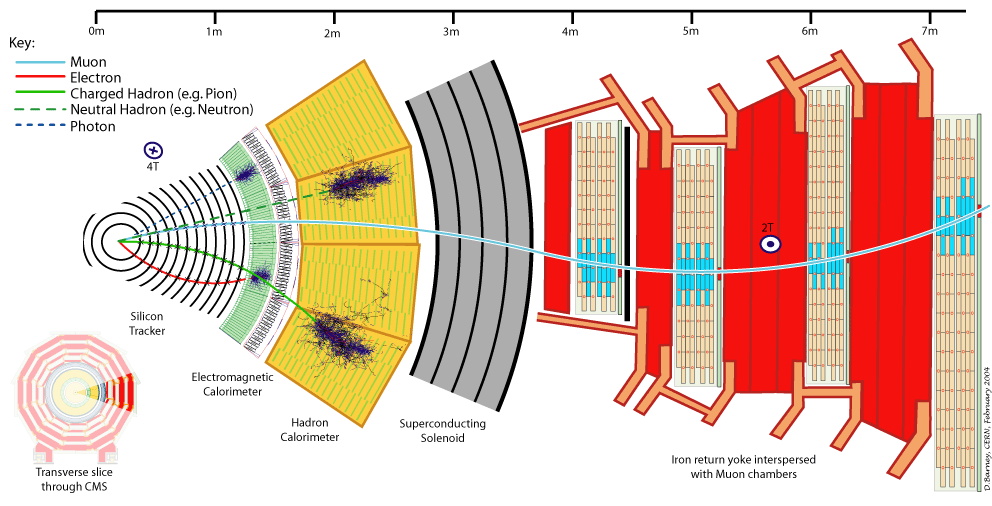
\includegraphics[width=15cm,height=7.5cm]{ch4/figures/cmsSlice.png}
\caption{Transverse view of the CMS detector, showing particle identification~\cite{Web:CERNcds}.}
\label{fig:cmsSlice}
\end{figure}

The CMS experiment makes use of various reconstruction algorithms~\cite{Lange:2011zza}, broadly divided into three steps as shown in 
\fig{\ref{fig:EvntRecons_BlockDiag}},  to interpret the raw digital information coming from the detector channels and yield the physics objects 
with associated charge, energy and position measurements, with these, in turn, to be used in a wide range of physics analyses. First, a local 
reconstruction in individual sub-detector modules is performed, which produces reconstructed hits (in short ``\emph{rechit}") representing position 
measurements in case of tracker and muon system, or clusters representing energy deposited in case of the calorimeters. Subsequently, information from 
different sub-systems, such as tracker, calorimeters, and the muon system, is used to reconstruct physics objects such as electrons from tracks; and 
photons and jets from calorimeter clusters, etc. Finally, a holistic approach, known as the particle-flow event reconstruction 
(PF)~\cite{CMS-PAS-PFT-09-001,CMS-PAS-PFT-10-001} is used, where information from all sub-detectors is linked in an attempt to individually and coherently
\begin{figure}[h]
\centering
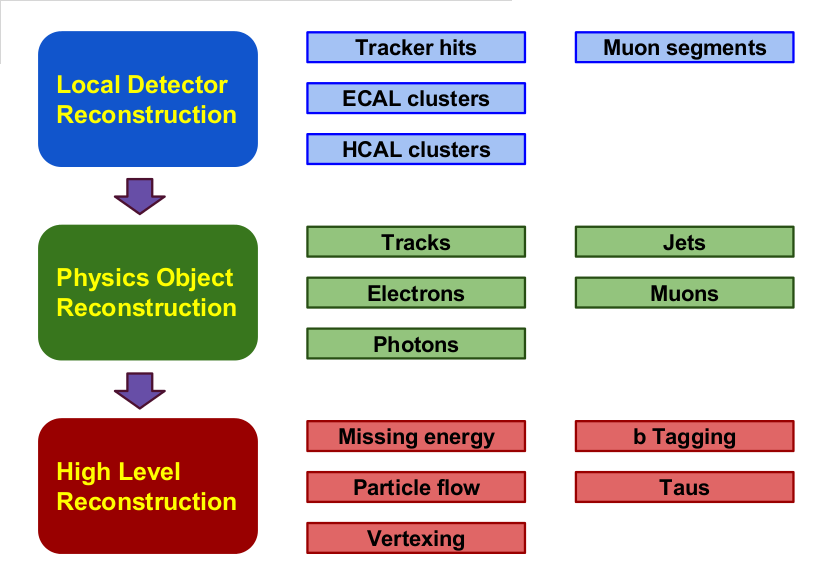
\includegraphics[width=13cm,height=9cm]{ch4/figures/EventReconstruction_BlockDiag.png}
\caption{Flowchart of event reconstruction algorithms.}
\label{fig:EvntRecons_BlockDiag}
\end{figure}
reconstruct and identify particles such as photons, leptons, pions, etc., in a given event. Composite objects, such as jets, \met, hadronically 
decaying $\tau$ leptons, are then finally created using these PF particles. 

In this chapter, we begin with the description of track reconstruction in the tracker system, followed by the primary vertex reconstruction. 
Then, we concentrate on describing the reconstruction and identification of photons and jets in the calorimeters, for these are the physics objects 
of interest used in ``Search for excited quarks in a photon and jet final state'', presented in this thesis. 

\section{Track Reconstruction}\label{sec:trackReco}
The reconstructed tracks of charged particles form the most fundamental objects in the reconstruction of collision events, subsequently 
contributing to the reconstruction of electrons, muons, taus, and hadronic objects as well as determination of primary interaction and 
displaced vertices. For each bunch crossing, few hundreds to a thousand charged particles travel through the CMS tracker system. In such
an environment, the tracking software aims to perform efficient reconstruction over a wide range of transverse momenta from 100\unit{MeV} to 
1\unit{TeV}, while keeping the misidentification rate low. These challenges are overcome by using the Combinatorial Track Finder (\gls{CTF}) 
algorithm~\cite{Adam:934067,Chatrchyan:2014fea} iteratively.

The tracking is done in several steps or iterations (6 in this case). The basic idea is to search for tracks with relatively large \pt,
produced near the interaction region. After each iteration, hits associated with tracks found in all preceding iterations are not considered
so as to reduce the combinatorial complexity and simplify subsequent iterations in the search for low-\pt tracks. Iteration-0 starts by reconstructing 
the highest quality tracks with $\pt>0.8\unit{GeV}$, identified as those having highest \pt, consistent with the primary vertex, and contain three 
pixel hits (indicating the track went through each layer of the pixel detector). In iteration-1, remaining high \pt tracks with only two pixel hits 
and close to the interaction point are reconstructed. Iteration-2 collects low \pt tracks originating from the primary vertex. These first three 
iterations reconstruct prompt tracks with an efficiency of $\sim90\%$ for charged hadrons and $\sim99.5\%$ for muons. Finally, Iterations-3 to 5 
reconstruct the tracks that originate outside the luminous region of the collision and are not found in previous iterations.

Each iteration is composed of four logical steps $-$ seed generation; pattern recognition or track finding; track fitting; and ambiguity
resolution or track selection. While we describe these below, further details can be found in Ref.~\cite{Chatrchyan:2014fea}. 
\begin{itemize}
\item \emph{Seed generation:} The seed defines the initial trajectory parameters and associated uncertainties of possible tracks. A track seed is 
built from either two or three hits in different layers of the pixel detector and is used to make an initial estimate of the trajectory parameters, 
\ie, track \pt, its position and associated uncertainties. The trajectory of charged particles follow a helical path.
\item \emph{Pattern recognition or track finding:} The Kalman filter algorithm\footnote{ Kalman filter is an estimation technique, that provides 
efficient means (recursively) to infer the state of a process, such that the mean squared error of the estimated parameter is minimized. The filter 
is so effective that it can estimate the parameters precisely even when the modelled system is unknown. More details about the same can be found 
in Ref.~\cite{Fruhwirth:1987fm}}~\cite{Fruhwirth:1987fm} makes use of the track parameters given by the trajectory seed for track finding. It 
extrapolates the trajectory of each track seed outwards by adding the collection of hits from successive layers of the tracker. The hits are fit
using the Kalman filter technique and a $\chi^{2}$ test as defined in Ref.~\cite{Chatrchyan:2014fea} is used to check the compatibility of 
the hits with the extrapolated trajectory.
\item \emph{Track fitting:} Once the candidate track has been found in the pattern recognition stage, tracks are fit again to remove any bias
introduced at the seeding step and obtain a final estimate of the trajectory parameters. First, a Kalman filter fit is performed on the first few 
hits of the track candidates. Then, the result of this fit and the innermost hit is used to initialize a Kalman filter fit to the entire track
candidate. The result is finally smoothed by averaging its result with a second fit performed in the reverse direction (the outermost hit to the 
innermost). A check is also done to find if there are any spurious hits (outliers) associated with the track. The outliers are found based on the 
probability that a pixel is consistent with the track, after taking into account the charge distribution of the hit in the pixel. The outlier hits 
are removed from the track, and the process is repeated until no outliers exist.
\item \emph{Track selection, or Ambiguity resolution:} In an event, there is a finite probability that the track finding procedure may yield a 
few fake tracks, namely reconstructed tracks not associated with charged partices. The fake rate (fraction of reconstructed tracks that are fake) 
can be substantially reduced by using certain quality requirements. Track quality criteria including requirement on the number of layers in a track, 
the $\chi^{2}$ per degree of freedom (number of tracker layers that have hits)  of the track, and its transverse and longitudinal impact parameters 
are used to remove fake tracks. After passing the above selection criteria, the track candidate is finally referred to as a track, or otherwise discarded.
\end{itemize}

\section{Reconstruction of Primary Vertices}
Interaction vertices or primary vertices (PV) are determined from the track collection. It is done in three steps. First, the tracks are selected, 
second, the clustering of tracks is done corresponding to a vertex, and finally, each group of tracks is fit to determine the position of the vertices. 

The location of the primary interaction vertex is reconstructed using pixel tracks with \pt in excess of 1\unit{GeV} and a transverse impact parameter 
less than 1\unit{mm} with respect to the beamspot~\cite{Miao:1061285}. These tracks are then clustered along the beam axis ($z$-direction) by requiring
a seperation of at least 1\unit{cm} between clusters. The clustering determines how many primary vertex candidates exists and how to assign the 
tracks to them. Finally, each cluster of tracks assigned to a primary vertex candidate is fit with the Adaptive Vertex Fitter (AVF)~\cite
{Fruhwirth:1027031} to determine the PV parameters, including its position. The AVF is an iterative Kalman Filter where tracks in each vertex are 
weighted according to their compatibility with the PV. This adaptive vertex fitter does not reject outlying tracks. Instead it down-weighs outliers
with a weight, given by:
\begin{equation}
w_{i}(\chi_{i}^{2})=  \frac{\text{exp}(-\chi^{2}_{i}/2T)} {\text{exp}(\text{exp}(-\chi^{2}_{i}/2T) + \text{exp}(-\chi^{2}_{c}/2T)) }
\end{equation}
where $w_{i}$ is the probability that a track, $i$ belongs to a vertex. The constant $\chi_{c}^{2}$ is the threshold where the weight has a value
1/2. Below this value, a track is considered a outlier. The variable $T$ is a parameter that controls the shape of the functional dependence. More
details of vertex reconstruction can be found in Refs.~\cite{Schmidt:1345323, Fruhwirth:1027031, Chatrchyan:2014fea}. The vertex candidates are finally
sorted in decreasing order according to the sum of their track $\pt^{2}$. The candidate with largest sum is consisdered as the primary vertex.
The PV resolution is $10-12\unit{\mu{m}}$ in all the three dimensions. 

\section{Photons}\label{Se:photonReco}
Photons produced in \pp collisions or from decay of other particles deposit their energy in the crystals of the ECAL via electromagnetic interactions. 
The photon reconstruction algorithms~\cite{Khachatryan:2015iwa} reconstruct the energy and momentum of the photon candidates from these ECAL crystals. 

\subsection{Photon Reconstruction}
The reconstruction of photons~\cite{Khachatryan:2015iwa} begins with the recovery of the energy deposited by them into the ECAL. In the absence of any 
material in-between the collision point and the calorimeters, about 97\% of the photon energy would be contained in a $5\times5$ cluster of the ECAL 
crystals. For electrons too, one uses a similar reconstruction technique with additional information from the tracker system. The presence of material 
in front of the ECAL causes electrons and positrons to undergo bremsstrahlung and photons to convert into $e^{+}e^{-}$ pairs. As bremsstrahlung 
emissions have effects analogous to that of pair-production, the same clustering algorithms are employed for both electron and photon reconstruction. 
The solenoidal magnetic field causes the energy reaching the ECAL to spread in the $\phi-$direction, whereas the distribution of energy in the $r-z$ 
plane is unaffected due the magnetic field. To account for this energy spread, electrons and photons are reconstructed from clusters of the ECAL 
crystals, called superclusters (\gls{SCs}). The main aim of the clustering algorithms is to group neighboring crystals to collect energy deposited 
by the electromagnetic shower in the ECAL. Two different clustering algorithms, namely, ``Hybrid Clustering algorithm" and ``Multi$5\times5$ algorithm" 
are used to find SCs, respectively in EB and EE, based on the differences in position and geometry of the 
crystals~\cite{Khachatryan:2015iwa,Khachatryan:2015hwa,Anderson:1365024}.

\subsubsection{Hybrid Algorithm}
The clustering in the EB region takes advantage of the $\eta-\phi$ geometry of the crystals. The algorithm~\cite{Khachatryan:2015hwa,Anderson:1365024} 
works by collecting  energy within a rectangular window spread in the $\phi-$direction, and crystals sorted in the decreasing order of \et. We 
give, below, a brief description of the algorithm.
\begin{itemize}
\item Hybrid clustering algorithm starts with a search for a seed crystal, defined as the crystal with the highest energy deposit, with the 
requirement that $E_{\mathrm{T,seed}} > \etxy{min}{seed}$. Clustering terminates if no such crystal is found.
\item Once the seed crystal is found, arrays of $1\times5$ crystals (also called dominos) with energies greater than $E^{\text{min}}_{\text{array}}$ 
are added in $\phi\times\eta$ plane around the seed crystal, in a range of $N_{\text{steps}}$ crystals in both directions of $\phi$.
\item The adjoining arrays are then grouped into clusters, where each cluster is required to have a seed array with energy in excess of 
$E^{\text{min}}_{\text{seed-array}}$ in order to be added to the final cluster, known as the supercluster (SC).
\end{itemize}
The values for various parameters used in the algorithm defined above are listed in \tab{\ref{Table:Hybrid}} and the procedure is illustrated in 
\fig{\ref{fig:Hybrid}}. 
\begin{table}[h]
\centering
\begin{tabular}{|l|c|}
\hline
Parameter & Value \\
\hline
\hline
\etxy{min}{seed}           & 1\unit{GeV} \\
%$E_{\mathrm{wing}}$    & 0\unit{GeV} \\
$N_{\text{steps}}$      & 17\unit{crystals} \\
$E^{\text{min}}_{\text{array}}$  & 0.1\unit{GeV} \\
$E^{\text{min}}_{\text{seed-array}}$    & 0.35\unit{GeV} \\
\hline
\end{tabular}
\caption{Parameter values used in Hybrid algorithm.}
\label{Table:Hybrid}
\end{table}
\begin{figure}[h]
\centering
\subfloat[A depiction of Hybrid Clustering algorithm used in EB region.]{\label{fig:Hybrid}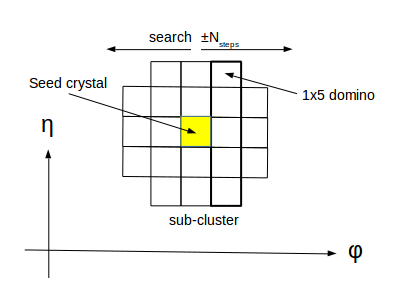
\includegraphics[width=10cm,height=5.5cm]{ch4/figures/ECAL_Hybrid_v2.png}}\\
\subfloat[Two overlapping Multi$5\times5$ clusters. Crystals with yellow colour can potentially seed further multi$5\times5$ clusters.]{\label{fig:Multi}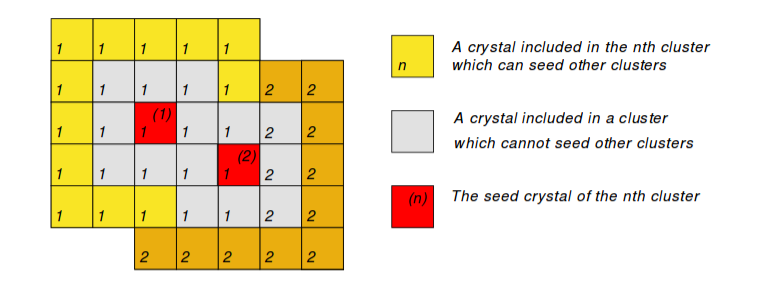
\includegraphics[width=13cm,height=5cm]{ch4/figures/ECAL_Multi5.png}}
\caption{Schematic overview of clustering algorithms in barrel and endcap ECAL regions~\cite{Anderson:1365024}.}
\label{fig:ECALClustering}
\end{figure}

\subsubsection{Multi$5\times5$ Algorithm}
The hybrid algorithm~\cite{Khachatryan:2015hwa,Anderson:1365024} can't be applied in the EE region, since unlike the EB region the crystals 
are not arranged in an $\eta-\phi$ geometry in this region. Thus, the Multi$5\times5$ algorithm, which tries to implement the same idea in a different 
fashion, is used. As described below, it also operates on crystals sorted in descending order in deposited \et.
\begin{itemize}
\item First, search for a crystal which does not already belong to a cluster and begin the clustering procedure with a seed crystal 
satisfying $E_{\text{T,seed}} > \etxy{min}{EEseed}$.
\item Check if the energy deposited in the seed crystal is a local maximum by comparing it to those deposited in the four nearest neighbors on 
each side in a Swiss Cross pattern. If it is not, go back to previous step.
\item Cluster a $5\times5$ matrix of crystals around the seed crystal, including only those crystals that do not already belong to a cluster. 
\item To collect overlapping deposition due to bremsstrahlung, the outer 16\unit{crystals} of the $5\times5$ matrix are allowed to seed new
matrices but the crystals already included in a cluster can not belong to another one. 
\end{itemize}
Finally, superclusters are built by summing up all the clusters satisfying $E_{\text{T,cluster}} > E^{\text{min}}_{\text{T,cluster}}$ and lying within 
a range $\eta\pm\Delta\eta_{\mathrm{road}}$ and $\phi\pm\Delta\phi_{\mathrm{road}}$ around each seed crystal. The parameter values used for this 
algorithm are listed in \tab{\ref{Table:Multi}} and its pictorial representation is shown in \fig{\ref{fig:Multi}}.
\begin{table}[h]
\centering
\begin{tabular}{|l|c|}
\hline
Parameter & Value \\
\hline
\hline
$E^{\text{min}}_{\text{T,EEseed}}$  & 0.18\unit{GeV} \\
$E^{\text{min}}_{\text{T,cluster}}$ & 1\unit{GeV} \\
$\Delta\eta_{\mathrm{road}}$ & 0.07 \\
$\Delta\phi_{\mathrm{road}}$ & 0.3\unit{rad} \\
\hline
\end{tabular}
\caption{Parameter values used in Multi$5\times5$ algorithm.}
\label{Table:Multi}
\end{table}

The ECAL endcap region, \ie, ($1.6<\abs{\eta}<2.5$) is covered by the ECAL preshower (ES) detector. Electrons and photons traversing in this
region deposit some of their energy in the preshower, so this energy needs to be measured and must be added to each cluster. 
To get the total energy of the showering particle for each super cluster the corresponding energy of the ES strips, found at the position of
intersection formed by extrapolating the position of the SC towards the interaction point, is added to it.

Regardless of the clustering algorithm, the position of the supercluster is estimated through a weighted average of the position of all the 
crystals, where each crystal contributes with a weight, $w_{i} = max(0,4.7\,+\,\ln(E_{i}/E_{SC}))$~\cite{Meschi:687345}. The superclusters 
are subsequently promoted to photon candidates and the direction of the photon momentum is estimated by connecting the position of the supercluster 
to that of the primary vertex in the event. If several primary vertices are found, the one with the highest scalar sum of track \ptx{2} is chosen.

\subsubsection{Energy Corrections}
Measuring the energy of electromagnetic objects with very high resolution is essential for precision measurement of the SM parameters and searches 
beyond the SM. A precise measurement of energy deposition in the calorimeters can also help improve measurement of \met, which is another important 
quantity for various new physics searches. Numerous factors can effect ECAL energy resolution, such as interaction of electromagnetic particles with 
the material of the tracker system, leading to bremsstrahlung and pair-production and, thus, energy loss. The role of the supercluster energy 
correction~\cite{Anderson:1365024} is to compensate for these energy losses and to control energy scales and achieve a homogeneous response 
in the full calorimetric volume. The reconstructed photon energy is given by:
\begin{equation}
E_{\gamma} = F_{\gamma}\times{G}\times\sum_{i=1..N}c_{i}\times{A_{i}}
\end{equation}
where, $A_{i}$ are the digital amplitudes in the ADC counts; $c_{i}$ are the inter-calibration terms that equalize the responses of the different
crystals; $G$ is the global energy scale defined in such a way that sum of amplitudes of a $5\times5$ crystal matrix multiplied by $G$ amounts
to the total energy of an incident uncoverted photon. The factor $F_{\gamma}$ represents a correction term to the supercluster energy and receive
contribution from three types of effects, as described below:
\begin{itemize}
\item {\bf Variation of shower containment} as a function of the position in the detector is parametrized by a function $C_{EB}(\eta)$. It is 
important only in the EB region, where the non$-$uniformities in the lateral shower leakage need to be corrected because of the off-pointing geometry
of the crystals. %These corrections are obtained from Monte Carlo simulations, with an overall contribution of about $\le1\%$ .
\item {\bf Variations in algorithm response} to different SC topologies are corrected through a function, $f_{brem}$, where, $brem$ is the 
energy loss due to bremsstrahlung, characterized by
\begin{equation}
brem = \frac{\sqrt{\sum_{i} \frac{E_{i}}{E_{SC}}(\phi_{i}-\phi_{SC})^{2}}}{\sqrt{\sum_{i}\frac{E_{i}}{E_{SC}}(\eta_{i}-\eta_{SC})^{2}}}
\end{equation}
where the sum $i$ runs over all the crystals in the SC and $\eta_{SC}, \phi_{SC}$ refers to the SC position. This function is almost 
insensitive, within certain limits, to the amount of material in front of the calorimeter. This contribution is $\lesssim7\%$ in the EB region,
and $\lesssim20\%$ in the EE region~\cite{Anderson:1365024}.
\item {\bf Residual variations} due to non-uniform distribution of material in the detector, and the energy dependence of the energy-collection
efficiency need to be corrected with a factor $f(\et,\eta)$.
\end{itemize}

\subsection{Photon Identification}\label{Se:photonId}
The most significant background to direct photon final state are QCD processes, where jets fragment to light neutral mesons, such as $\pi^{0}$ and 
$\eta$, which, subsequently, decay into a pair of overlapping photons. Thus, in order to maintain purity of the photon signal selection, 
the separation of the prompt photon component from this background at high energies must be done with great purity. 

Even though an event-by-event discrimination of signal photons from the background is not possible, a separation of signal and background is possible 
on a statistical basis. An effective instrument used to segregate signal from background is based on the topology of the deposited energy in the
calorimeter. Several variables sensitive to differences between signal and background photons can be constructed and are classified under the heading
``shower shape variables". The electromagnetic shower from neutral mesons contributing to the background are produced in jets, and thus are always 
surrounded by some hadronic activity. The resultant showers are wider than one produced from a prompt photon because of the overlapping nature of two 
showers merging into one from two photons emanating from neutral meson. The jet backgrounds can, therefore, be reduced by requiring the reconstructed 
supercluster in the ECAL to be isolated, \ie, limiting the amount of energy carried by other particles surrounding them. The following sections briefly 
describes different types of variables used to identify and isolate prompt photons.

\subsubsection{Shower shape variables}\label{section:ShowerShapeVariables}
The shower topology is an important discriminator to distinguish prompt photons from photons coming from neutral mesons. Several variables can be 
computed to parametrize the differences between the events due to prompt photons and those coming from neutral hadrons in jets.
\newline
{\bf Hadronic over Electromagnetic ratio (H/E) : } It is defined as the ratio of the energy deposited in the HCAL behind the photon supercluster and 
the photon energy as measured by the ECAL. The ratio H/E is the energy deposited in the single closest HCAL tower to the supercluster position 
inside a cone of radius 0.15 in the $\eta-\phi$ plane centered on the photon direction to the energy deposited in the ECAL for that supercluster. 
Since the ECAL has sufficient depth (measured in $X_{0}$) to contain the shower within it and the probability of shower leakage into the HCAL is 
very small, this is a good discriminator.
\newline
{\bf Rectangular ratios : }  The hypothesis of a single photon shower against multiple overlapping showers can be tested by searching for a double
peak structure in the topology of the supercluster. The simplest of variables sensitive to this feature can be computed as the ratio of energy 
deposited in a $n\times{m}$ crystal window around the supercluster seed crystal to the energy deposited in a $n'\times{m'}$ window  or the total
supercluster energy. Two such variables used are called $R_{1}$ and $R_{9}$, where $R_{1}$ is defined as the ratio of seed crystal energy to the 
supercluster energy while $R_{9}$ is the ratio of energy deposited in a $3\times3$ window to the supercluster energy.
\newline
{\bf Shower profile : } A sophisticated way to look at a possible double peak structure is to determine the lateral extension of energy deposits in the 
$\eta-$direction. A variable, \sigmaIetaIeta, defined as the energy weighted standard deviation of a single crystal $\eta$ within a $5\times5$ 
crystal lattice centered at the crystal with maximum energy, gives the transverse shape of the electromagnetic cluster. It is computed with 
logarithmic weights and is expressed as:
\begin{equation}
\begin{split}
\sigma_{i{\eta}i{\eta}}^{2} =  &\frac{{\sum}(\eta_{i}-\bar{\eta})^{2}w_{i}}{{\sum}w_{i}}, \\
                           &\text{where}\:\:\bar{\eta} = \frac{{\sum}w_{i}\eta_{i}}{{\sum}w_{i}} \:\:\: \text{and} \:\: w_{i} = \text{max}\left[0 \: ;\: 4.7+\text{log}\left(\frac{E_{i}}{E_{5\times5}}\right)\right]
\end{split}
\end{equation}
where the sum runs over the $5\times5$ crystal matrix around the most energetic crystal in the supercluster, and the $\eta$ distances are measured in 
units of the crystal size in the $\eta-$direction. This variable helps in discriminating the clusters belonging  to the prompt photon for which the 
distribution is narrow and symmetric when compared to misidentified photons, for which there is a tail in the lower side of the distribution.
\newline
{\bf Conversion safe electron veto : } This variable requires that there be no charged particle track with a hit in the pixel detector not matched to a 
conversion vertex~\cite{Khachatryan:2015iwa}, pointing to the direction of photon cluster in the ECAL. It helps to distinguish photons from electrons.

\subsubsection{Isolation based variables}\label{Se:photonIso}
The fact that prompt photons arising from the interaction vertex are not produced in association with other particles can be used to construct 
various isolation sums. The signal
photon candidates can be extracted by simply allowing a maximum threshold to the amount of allowed activity surrounding the photon candidates
in various sub detectors. These isolation sums can be expressed as the total amount of energy/momentum carried by particles estimated using 
particle flow algorithm, surrounding the photon candidate. Three types of sums : the total energy carried by the charged hadrons, the neutral 
hadrons and the photons, have been employed in this thesis. All the three sums are evaluated in a cone of radius $R=\sqrt{\deta^{2}+\dphi^{2}} = 0.3$ around the photon candidate. Respective veto regions are defined for each isolation sum, with the motive to isolate the energy deposits due to the
photon candidates. 
\newline
{\bf Particle Flow Charged Hadron Isolation: } Sum \pt of all charged hadrons within a hollow cone of $0.02<\dR<0.3$ around the supercluster to 
isolate showers arising from non-converted or late converted photons having no associated track in the tracker system.
\newline
{\bf Particle Flow Neutral Hadron Isolation: } Sum \pt of all neutral hadrons within a cone of $\dR=0.3$ around the supercluster because the 
clusters having energy deposition from neutral hadrons will lead to a broader distribution of energy compared to isolated photons, as well as 
leakage in the HCAL.
\newline
{\bf Particle Flow Photon Isolation: } Scalar sum \pt of all photons within a cone of $\dR=0.3$ excluding a strip in $\eta$ of 0.015 around 
the supercluster, to seperate from converted photons going in to $e^{+}e^{-}$ and having a broader spread in $\eta-$direction.

\subsubsection{Anomalous ECAL energy deposits}\label{Se:Spikes}
Anomalous energy deposits (such as noise) in the ECAL are a source of background while identifying photons from \pp collisions. These deposits 
of energy are caused by direct ionization of an Avalanche Photo-diode (APD) by a highly ionizing particle such as a proton~\cite{CMS-NOTE-2010-012}. In such 
a case, the entire energy is deposited in a single crystal and this is referred to as a ``spike". The rate of these spikes scales with $\sqrt{s}$ at 
a level which is consistent with the increase in charged particle multiplicity from \pp collisions~\cite{Khachatryan:2010us}.

The pulse shape of a signal and timing of the shower development in the ECAL allows distinction between the energy deposits by true electromagnetic 
showers and those from direct ionization of an APD. While the ``spikes'' due to electronic noise in APD peaks instantaneously and deposits most
of the energy in a single crystal, the signal from electromagnetic showers take time to develop and attain a maximum spread over several crystals.
%As an example, signals from electromagnetic showers are peaked at a time of zero (relative to \pp collision time), 
%while for ``spikes'', it is peaked at about -10\unit{ns}. The difference in time is because the electromagnetic shower takes time to develop and 
%attain a maximum, while direct ionization of an APD results in a much shorter rise-time.

\subsubsection{Beam Halo}
Protons from LHC beams may collide with atomic nuclei of gas atoms or other material along the beam line. 
These interactions results in a ``halo" of particles which tend to be nearly parallel to the beam direction. These ``halo" particles are
composed of mainly baryons, mesons, and muons. Muons from beam halo can penetrate through large amounts of detector material including the 
endcaps of the CMS. These muons may also interact with material in CMS and create photons from bremsstrahlung. The resulting photons from these
interactions can be detected by the ECAL and tend to be relatively isolated. Photons coming from \pp collisions at the interaction 
point are reconstructed with a $t_{seed}$\footnote{$t_{seed}$ is the timing of the seed crystal, the highest energy crystal in the cluster.}$\approx0$, 
while those resulting from beam halo tend to have a negative $t_{seed}$.

\section{Jets}\label{Se:Jet}
The quarks and gluons jets have played an important role in establishing QCD as the theory of the strong interactions within the SM. A jet is 
referred to as collimated spray of hadrons, reflecting the configuration of quarks and gluons at short distances. Thus, by analysing the energy
and angular distributions of the jets, the properties of the strong forces acting between them can be studied. Clustering the energy deposits 
or momentum measured by tracker system from a large collection of particles into one or more jets is done by a jet clustering algorithm. 
Jet reconstruction algorithms provide a set of rules, based on proximity, for clustering of particle tracks or calorimeter towers into jets. A good 
jet reconstruction algorithm needs to address the following set of issues:
\begin{itemize}
\item It should be simple and easy to implement in an experimental analysis and theoretical calculations and should be independent of detector structure.
\item It should yield a finite cross section at any order in perturbation theory and also be relatively insensitive to hadronization effects.
\item It should be infrared and collinear safe.
\item It should be fully specified, including defining in detail any pre-clustering, merging and splitting.
\end{itemize}
Infrared and collinear safety is a fundamental requirement for jet algorithms. Infrared safety ensures that adding a soft gluon would not
effect the jet clustering results while collinear safety take cares that the splitting of one parton into two partons leads to similar
results in jet clustering. The configurations of infrared and collinear safety are shown separately in \fig{\ref{fig:JetCones}}.
\begin{figure}[h]
\centering
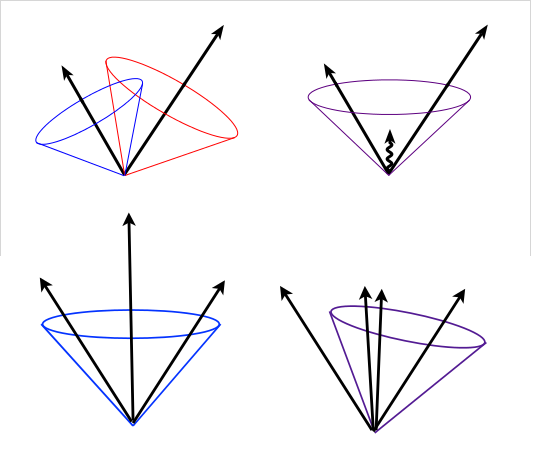
\includegraphics[width=10cm,height=8cm]{ch4/figures/JetCones.png}
\caption{Infrared safety (top) : Addition of a soft gluon. Collinear safety (bottom) : Splitting of one parton into two collinear partons.}
\label{fig:JetCones}
\end{figure}
For the analyses presented in this thesis, jets are reconstructed and identified using the ``particle-flow" (PF)~\cite{CMS-PAS-PFT-09-001} event
reconstruction and \antikt jet~\cite{Cacciari:2008gp} clustering algorithm, which are described in brief detail in the sections to follow. 

\subsection{Particle Flow Reconstruction}\label{Se:PFAlgo}
The ``particle flow" (PF)~\cite{CMS-PAS-PFT-09-001} approach is an attempt to identify and reconstruct individually each particle originating 
from the \pp collisions via coherent use of all sub-detectors. The PF algorithm is designed to maximally exploit the high efficiency tracking 
and high granularity calorimetric (especially ECAL) system of the CMS detector. The PF jets are composed of individually identified charged 
hadrons, photons, electrons, and neutral hadrons in the barrel region, \ie, within the reach of the ECAL and the tracker. It leads to an optimal 
determination of the direction, energy, and type of particle in each event. The PF algorithm consists of mainly three steps.

The \emph{first step} begins with making \emph{building bricks/elements} of the PF algorithm, \ie, reconstruction of charged particle tracks 
and clusters of calorimeter energy deposits. Tracks are obtained as described in \sectn{\ref{sec:trackReco}}, while the clusters are built using a
 dedicated PF clustering algorithm tuned to achieve high detection efficiency. The clustering procedure starts with a search for seeds, which 
correspond to energy deposits in calorimetric channels with a local maxima. The nearest neighboring channels are then added to it, forming 
\emph{topological clusters}. Energy deposits in each calorimeter channel is required to be above predetermined thresholds both for ECAL and HCAL
 in order to avoid contributions from electronic noise fluctuations. Finally, the positions and energies of clusters are determined iteratively 
by re-weighting the individual channel contributions as per the channel-cluster distance~\cite{CMS-PAS-PFT-10-003}.

The \emph{second step} constitutes the reconstruction of PF \emph{blocks} in the PF event reconstruction. As a single particle impinging the detector
can result in multiple PF \emph{elements} in the form of clusters and tracks, and in order to eliminate the possibility of double counting 
within the PF collection, they need to be connected via a mechanism called \emph{link algorithm}. All the tracks are extrapolated starting
from the last hit measured in the tracker system, to the ECAL and HCAL, at depths compatible with the electron and hadron shower profile
respectively, and clusters that are found to include the extrapolated tracks within their boundaries, are linked to the track. 
A link between ECAL (including the preshower detector) and HCAL clusters is also made when the position of the cluster in ECAL lies within
the envelope of the HCAL cluster. Going further, tracks from the tracker system are also linked to the tracks in the muon system forming the 
global and tracker muon candidates. A resultant block is usually composed of $\le$ 3 elements, and the quality of a block is defined by 
the compatibility of its constituent elements, either as the $\eta-\phi$ distance in the case of track-to-cluster and cluster-to-cluster links or 
a global fit $\chi^{2}$ for track-to-muon-track links. The limited size of each PF block renders the PF particle identification performance almost 
independent of event complexity~\cite{CMS-PAS-PFT-09-001}.

The \emph{third step} refers to the reconstruction and identification of each PF particles based on these PF \emph{blocks}.
The detailed reconstruction in the context of each particles is explained in~\cite{CMS-PAS-PFT-09-001}.

\subsection{\boldmath$\Antikt$ Clustering Algorithm}
The \antikt algorithm~\cite{Cacciari:2008gp} is an infrared and collinear safe clustering algorithm used as the default jet reconstruction algorithm. 
The \antikt is a special form of \kt algorithm~\cite{Catani:1993hr}, that is a clustering based, sequential recombination algorithm.
For a given set of input objects, it evaluates two distance measures for each object, namely, the distance \emph{d}$_{ij}$, between 
\emph{i}$^{\mathrm{th}}$ and \emph{j}$^{\mathrm{th}}$ objects, and the distance \emph{d}$_{iB}$, between the \emph{i}$^{\mathrm{th}}$
object and the beam line $B$, shown in \eqn{\ref{eq:ktAlgo1}} to~\ref{eq:ktAlgo2}.
\begin{eqnarray}
\label{eq:ktAlgo1}
d_{ij} & = & min(k^{2}_{\mathrm{T}i}, k^{2}_{\mathrm{T}j}) \frac{\dR^{2}_{ij}}{R^{2}} \\
d_{iB} & = & k^{2}_{\mathrm{T}i} \\
\label{eq:ktAlgo2}
\dR^{2}_{ij} & = & (\eta_{i} - \eta_{j})^{2} + (\phi_{i} - \phi_{j})^{2}
\end{eqnarray}
where \kt is the object transverse momentum, $\eta$ and $\phi$ are object pseudo-rapidity and azimuthal angle, respectively, and $R$ is the
predefined jet radius. The functioning of \kt algorithm can be briefly summed up as follows:
\begin{itemize}
\item Make list of particles and compute distances $d_{ij}$ and $d_{iB}$.
\item If $d_{ij}$ is smaller, entities \emph{i} and \emph{j} are combined into a jet and return to first step.
\item Otherwise, if $d_{iB}$ is smaller, the entity \emph{i} is pronounced as jet and removed from the list and return to first step.
\item Repeat until no particles are left.
\end{itemize}
The distance measurement can also be generalized as,
\begin{eqnarray}
d_{ij} & = & min(k^{2p}_{\mathrm{T}i}, k^{2p}_{\mathrm{T}j}) \frac{\dR^{2}_{ij}}{R^{2}} \\
d_{iB} & = & k^{2p}_{\mathrm{T}i}
\end{eqnarray}
where, $p$ is the parameter that is 1 for \kt algorithm and it implies that soft particles are clustered first. When $p = -1$, it refers to the \antikt 
algorithm, and in this case hard particles are clustered first rather than soft particles. For $p = 0$, an energy independent clustering algorithm  
known as Cambridge/Aachen (CA) algorithm~\cite{Dokshitzer:1997in} is obtained. The behaviors of different jet algorithms are illustrated in 
\fig{\ref{fig:JetClusteringAlgo}}. \Fig{\ref{fig:JetClusteringAlgo}} also illustrates SISCone jet algorithm that is based on the search for stable
cones. Other than being infrared and collinear safe, the \antikt jet algorithm also gives the best shape which helps in applying topological 
selections. The CMS supports \antikt algorithm with cone sizes $R=0.5$ and $R=0.7$.
\begin{figure}[h]
\centering
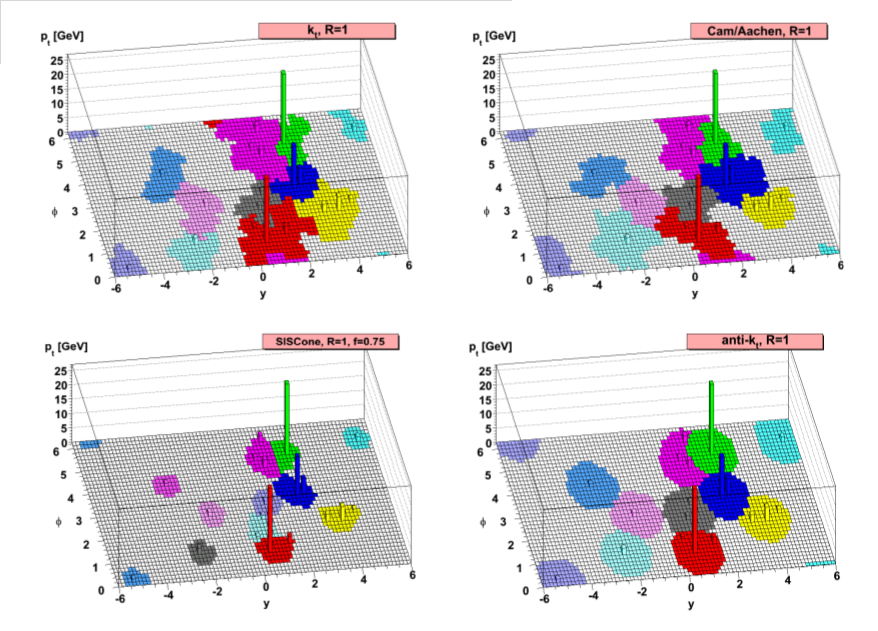
\includegraphics[width=13cm,height=10cm]{ch4/figures/JetClusteringAlgo.png}
\caption{The behaviors of different jet algorithms in parton level~\cite{Cacciari:2008gp}.}
\label{fig:JetClusteringAlgo}
\end{figure}

\subsection{Jet Energy Calibrations}\label{Se:Jec}
Energy measurement of the reconstructed jet is, typically, different from the corresponding true particle jet energy, owing mainly to non-uniform and 
non-linear response of the calorimeters. In addition, electronic noise and event pile-up too add to the discrepancy in energy measurement. The 
motive of jet energy correction (JEC) is to relate, on an average, the jet energy measurement in the detector to the energy of the corresponding 
particle jet. For jet energy correction, a multi-level factorized approach is undertaken, where each correction has a unique effect and is applied 
in a fixed order~\cite{CMS-PAS-JME-07-002}. These corrections are derived both from data-driven and MC-truth methods for \emph{in-situ} calibration. 
exitThe correction factors listed below are applied to the jets in a sequential manner. 
%The jets considered in the results presented later in thesis, are corrected using the following factors, in the order they appear below :
\begin{itemize}
\item L1 Offset : It is required to remove energy contribution coming from pile-up and underlying events~\cite{Cacciari:2007fd}. 
The median jet \pt is used to compute the energy density arising from these effects for each event, which is then multiplied by 
the jet area before subtracting it from the jet \pt.
\item L2 Relative ($\eta$) : It is a relative correction applied to the pile-up subtracted jet energy, to make the jet response flat
as a function of pseudorapidity.
\item L3 Absolute (\pt) : Once the jet energy has been corrected for $\eta$ dependence, another correction is applied to make the 
jet response flat in \pt also.
\item L2L3 Residual : Finally, after all above corrections, a factor is applied only to data events to deal with small,
residual difference between the data and MC, based on the \emph{in-situ} measurements of the relative and absolute jet energy scales.
\end{itemize}

\subsection{Jet Identification}\label{Se:JetID}
Once the jet has been reconstructed and all the corrections applied, it is now important to identify good reconstructed jets and to discriminate them
 from the fake jets due to electronic noise or other detector artifacts. For this job, a set of variables has been defined~\cite{Web:JetId}, which
 are listed below:
\begin{itemize}
\item Charged hadron fraction $-$ fraction of energy deposited by the charged hadrons in the HCAL.
\item Neutral hadron fraction $-$ fraction of energy deposited by the neutral hadrons in the HCAL.
\item Charged electromagnetic fraction $-$ fraction of energy deposited in the ECAL by the charged constituents of the jet.
\item Neutral electromagnetic fraction $-$ fraction of energy deposited in the ECAL by the neutral constituents of the jet.
\item Number of constituents or number of particles in the jet.
\item Charged multiplicity $-$ number of charged particles (charged constituents) in the jet.


\end{itemize}

%%\bibliography{ch4/ch4_ref}
